\item
\mbox{}
\begin{center}
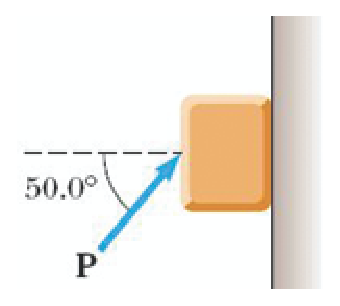
\includegraphics [scale=0.6]{./latex/eps/1_5_14_image_1.eps}
\end{center}

Balok dengan massa 3.00 Kg ditekan ke atas pada dinding dengan gaya \textbf{P} yang membentuk sudut $50^{0}$ terhadap horizontal. Koefisien gesek statik antara balok dengan dinding sebesar 0.25. Tentukan nilai yang mungkin dari besar gaya \textbf{P} agar balok tetap stasioner.

\begin{description}
    \item[Solusi:]
        \mbox{}
\begin{center}
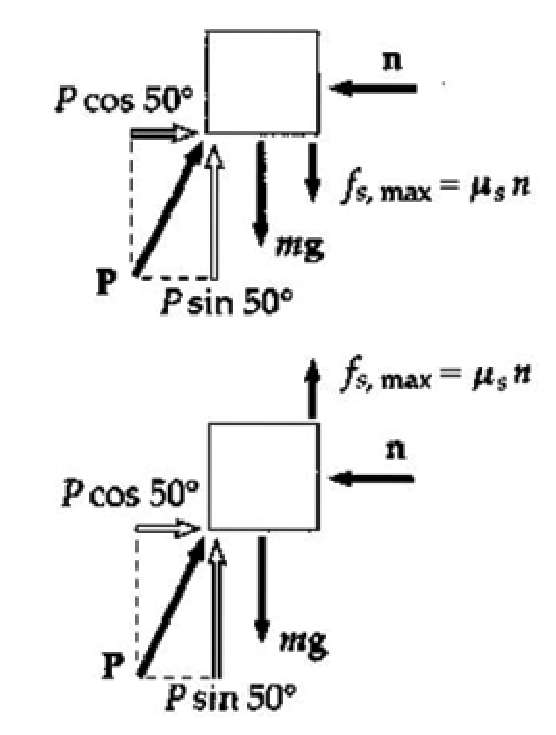
\includegraphics [scale=0.4]{./latex/eps/1_5_14_image_2.eps}
\end{center}

Kondisi saat balok akan naik ke atas. \\
\begin{eqnarray*}
\Sigma F_{x}=0 ;\quad P\cos 50^{0}-n&=&0 \\
f_{s,max}=\mu_{s}n: \quad f_{s,max}&=&\mu_{s} P \cos 50^{0} \\
&=& 0.250(0.643)P=0.161P
\end{eqnarray*}
\begin{eqnarray*}
\Sigma F_{y}=0;& &\quad P\sin 50^{0}-1.61P-3.0(9.8)=0 \\
P_{max}&=&48.6 N
\end{eqnarray*}
Kondisi saat balok akan jatuh ke bawah. \\
\begin{eqnarray*}
f_{s,max}&=&0.161P  \\
\Sigma F_{y}& &:\quad P\sin50^{0}+0.161P-3.0(9.8)=0 \\
P_{min}&=&31.7 N
\end{eqnarray*} 

\end{description}
